\chapter{Scope \\
%\small{\textit{-- Team-11}} 
\index{Chapter!Scope}
\index{Scope}
\label{Chapter::Scope}}
This ConOps document is intended to describe the machine learning model "ClauseGuard," designed to assist stakeholders in identifying deceptive clauses in terms and conditions (T\&C) contracts. This document follows the Concept of Operations template as laid down by the IEEE Guide for Information Technology—
System Definition—Concept of
Operations (ConOps) Document. This document aims to provide stakeholders who will be using the system with insights into its operation and functionality. 


\section{Identification\label{Section::Project Identification} }
This document is based on the system "Clauseguard" which is a machine learning model, trained to detect harmful clauses in terms and conditions (T\&C) Contracts.



\section { Document Overview \label{Section::Document Overview} }
This document outlines the concept and operations of the system "Clauseguard". It provides a detailed overview of the system, its intended operation, Justification for the the system, and operational policies. Furthermore, it details the working of the system, the end objective of the system, and the stakeholders. Finally, this document also details the impact of the system on the wider world. 


\section{System Overview\label{Section::System Overview}}

ClauseGuard is a machine learning model designed to assist stakeholders in avoiding deceptive clauses in terms and conditions (T\&C) contracts by analyzing the contents of the contract. A final result, similar to tools such as a plagiarism checker, will be displayed to the user, providing an indicator percentage of the number of deceptive instances identified by the algorithm. For each flagged detail, the system will provide a brief description explaining why it was flagged. The choice to sign the document will be left up to the discretion of the user.

ClauseGuard will be deployed on a web platform accessible to stakeholders from any geographic location. The diagram given below provides a high-level view of the system's operation.

\begin{figure}[h]
\centering
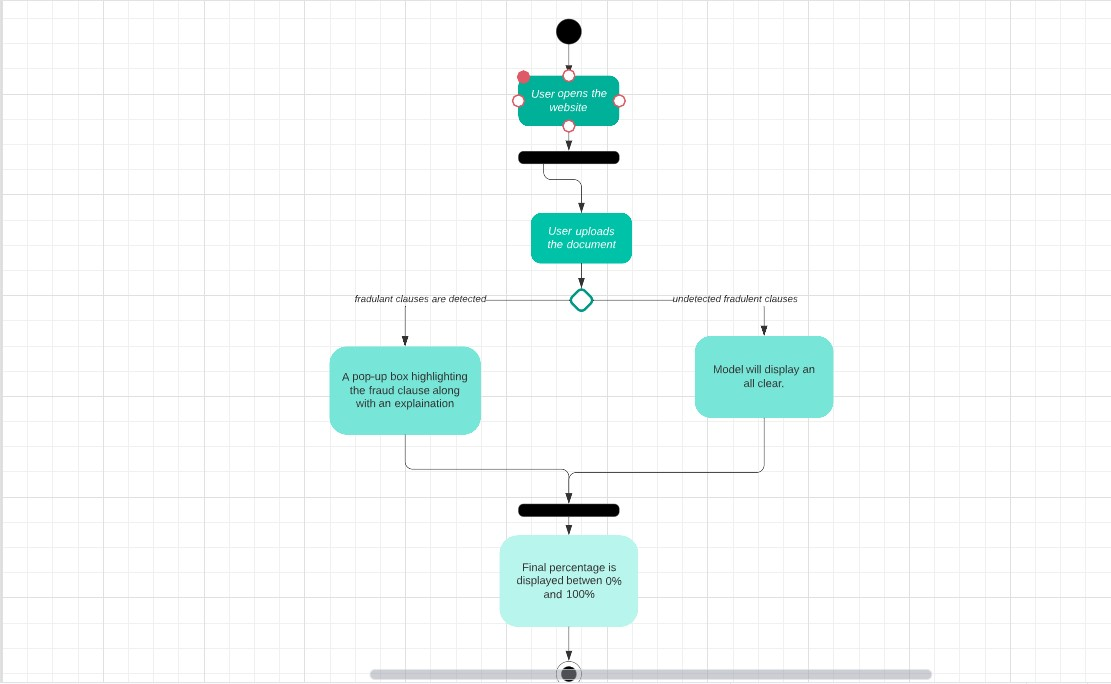
\includegraphics[scale=0.93]{Figures/activity diagram.jpg}
\caption{High-level overview of the system \ref{fig:system_overview}}
\label{fig:system_overview}
\end{figure}


% The primary goal of this project is to develop a machine learning model that assists stakeholders in avoiding deception by clauses in terms and conditions (T\&C ) contracts. This approach will automatically analyze all clauses within the contract, providing stakeholders with the necessary information to decide whether to proceed or not.
% Several popular machine learning libraries, such as scikit-learn \cite{scikit-learn}, the Natural Language Toolkit (NLTK) \cite{nltk}, and Keras \cite{keras}, will be utilized to create the model. Flask \cite{flask} and Django \cite{django} will be employed to develop the web application, enabling users to upload T\&C contracts in text or PDF formats and evaluate the presence of any deceptive clauses. Scikit-learn, NLTK, and Keras are widely used libraries for machine learning tasks.
% We will start by selecting a dataset of T\&C contracts that have been identified as containing fraudulent or unclear clauses. The scikit-learn and Keras libraries will be used for feature extraction, where we can extract relevant information from the text. After extracting the features, we can use them to train a machine learning AI model using the scikit-learn engine.
% Once the AI model is trained, it can be evaluated using the Keras library to determine its accuracy. If the model performs well, it can be used to identify whether clauses in T\&C contracts are fraudulent or unclear.
% In summary, this project aims to create a machine learning model that helps stakeholders avoid deception in T\&C contracts by automatically analyzing the clauses within the contract. By using popular libraries and web development frameworks, the model will provide stakeholders with valuable insights and help them make informed decisions about whether to proceed with an agreement or not.

% \begin{figure}
% \centering
% \scalebox{0.53}{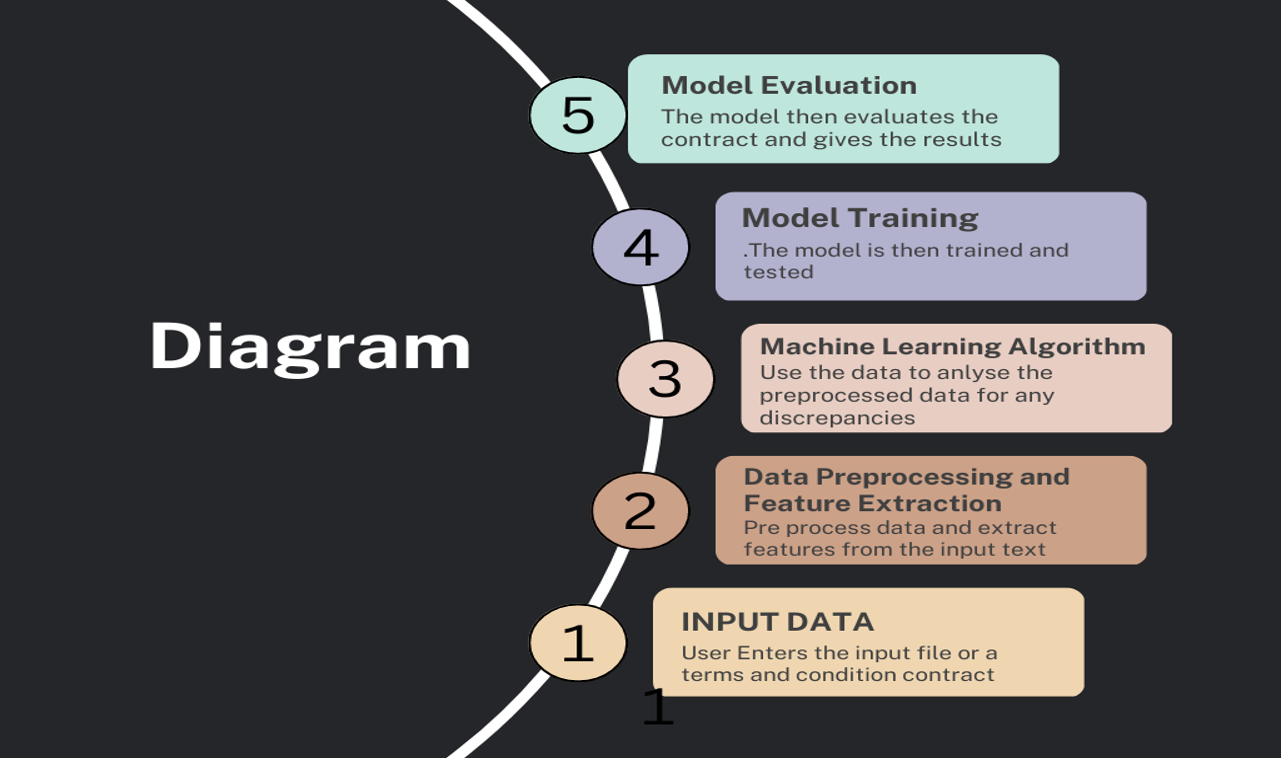
\includegraphics{Figures/Diagramoftheproposedsystem.png}}
% \caption{\label{Figure::Diagram Of The Proposed System} Diagram Of The Proposed System  \ref{Figure::Diagram Of The Proposed System}}
% \end{figure}
